\newpage
\section{Comments and Notes}\label{sec:04_comments}
% Intro
This section describes the problems encountered during the development of the application.


\subsection{Deploying the WebApp manually}\label{sec:04_comments_webapp}
% What
\Sec{sec:03_depl_webapp} describes how to start the \textit{WebApp} project using IntelliJ. Another solution would be, to create the \texttt{.war} artifact, and deploy that artifact to Apache Tomcat manually.

\subsubsection{Build and Deploy the WebApp Artifact}\label{sec:04_comments_webapp_artifact}
% Build
To create the \texttt{.war} artifact, the command \texttt{\$ mvn clean package} has to be executed in the root of the \textit{WebApp} project directory.
After the artifact has been built, it is located at \path{WebApp/target/marcel-stolin-web-app.war}, as shown in \Fig{fig:04_comments_webapp_artifact_created}. Next, to deploy the artifact to Apache Tomcat, it needs to be copied to the path \path{$TOMCAT_HOME\webapps}, where \texttt{\$TOMCAT\_HOME} is the directory of Apache Tomcat. This process is shown in \Lst{lst:04_comments_webapp_artifact_deploy}.

% Figure
\begin{figure}[h]
\centering
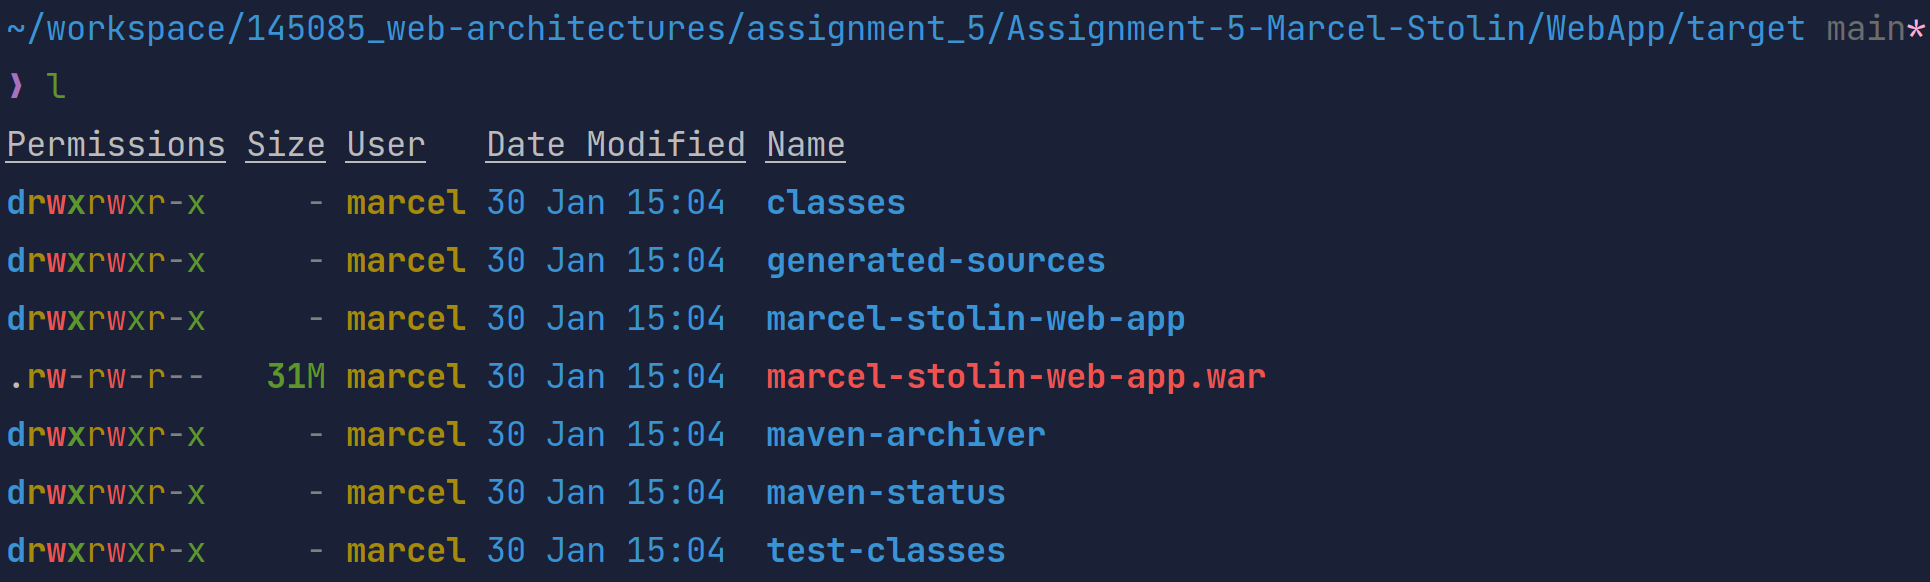
\includegraphics[scale=0.2]{images/04_comments/webapp-artifact}
\caption{\textit{WebApp} \texttt{.war} artifact}
\label{fig:04_comments_webapp_artifact_created}
\end{figure}

% Deploy
\begin{lstlisting}[label=lst:04_comments_webapp_artifact_deploy, caption=Artifact deployment command, language=sh]
$ cp target/marcel-stolin-web-app.war $TOMCAT_HOME/webapps
\end{lstlisting}

\subsubsection{Configure Apache Tomcat}
% Change port
As described in \Sec{sec:03_depl_webapp}, the port of Apache Tomcat needs to be changed to port 8000. Therefore, the file \path{$TOMCAT_HOME/conf/server.xml} has to be changed as given in \Lst{lst:04_comments_webapp_artifact_config}. This will change the default port to 8000.
% Server config
\begin{lstlisting}[label=lst:04_comments_webapp_artifact_config, caption=Apache Tomcat configuration, language=xml]
<Service name="Catalina">
  <Connector port="8000" protocol="HTTP/1.1"
             connectionTimeout="20000"
             redirectPort="8443" />
</Service>
\end{lstlisting}

% Start server
After the artifact has been deployed, and the default port is updated, the Apache Tomcat server can be started using the command \texttt{\$TOMCAT\_HOME/bin/catalina.sh start}. Then, the \textit{WebApp} is available at \url{http://localhost:8000/marcel-stolin-web-app}.
